% !TEX program = xelatex
% !BIB program = bibtex
% !Mode:: "TeX:UTF-8"
\documentclass{mcmthesis}
\mcmsetup{CTeX = true,   % 使用 CTeX 套装时,设置为 true
	tcn = 1923999, problem = D,
	sheet = true, titleinsheet = false, keywordsinsheet = false,
titlepage = true, abstract = false}
\usepackage{palatino}

\usepackage{lipsum} %添加lipsum宏包,就是随机生成一段文本,可以不使用
% \usepackage{boxie} %添加lipsum宏包,就是随机生成一段文本,可以不使用

\usepackage[UTF8, nocap]{ctex} %如果想使用中文输入的话,可以增加该宏包

\usepackage[framed,numbered,autolinebreaks,useliterate]{mcode}
 %正文摘要和控制页摘要名字修改
%\def\abstractname{Abstract}
\def\sheetsummaryname{Emergency Evacuation Simulation Model Based on Cellular Automata}



\begin{document}

 %控制页摘要内容

\begin{sheetsummary}
	\indent The threaten of terror attacks is getting progressively bigger, making the public worried about the safety in public resorts, such as the Louvre. A review of the evacuation plan to address different emergencies is in urgent need.  \\
	\indent In order to explore the preferable solutions, we first build the evacuation simulation model based on the two-dimensional cellular automaton. The main affecting factors of the leaving process are the structure of building and the detailed information of visitors. The two factors are formulated and quantized respectively. As the preparations for the model, we evenly divide the  building plane into grids and endow them with different numerical values according to the location.  The simulation is completed by the continual iterations of the grids' values. As for the iteration, we set several rules to emulate the actual movement of people, including movement rules, conflict avoidance rules and the emergency rules.  \\
	\indent Taking the randomness of individual choice and emergency into consideration, it is hardly possible to point out a universal optimal evacuation plan. So we  define two indexes to evaluate different plans: swiftness and safety. They are formulated respectively by the lasting time of the departure process and the occurrence times of emergency. The evaluation model is the combination of the two indexes. \\
	\indent Utilizing the simulation model and the evaluation criteria set up above, we explore a broad set of options for various conditions. With regard to the Louvre, we offer four suggestions, consisting of the maximum number of visitors, the reasonable distribution of exhibition halls, the strategy to utilize the hidden exits as well as the route planning of the emergency personnel. \\
	\indent As for the utilization of the hidden exits, the optimal location is away from the exit or the staircase. The reasonable strategy is opening up the hidden exit only when the density around the exit is less than 0.5, in order to decrease the possibility of random confusion. \\

	\indent \textbf{Keywords:} Cellular Automata; emergency evacuation simulation model; evaluation optimization;
\end{sheetsummary}
 %关键词
 % Generate the Table of Contents, if it's needed.
\maketitle
\tableofcontents
\newpage


\section{Introduction}
Nowadays, tourism has been one  essential part of the daily life. As the most famous and favorable tourist attraction, the Louvre, located in Paris,  receives more than 8 million visitors each year. The high occurrence rate of terror attacks results in highly concerns of the safety problems in many popular resorts. It is evident that a review of the  emergency evacuation plans  is in urgent need. The general goal of the plan is to accomplish the evacuation of all the visitors, meeting the requirements of safety and swiftness.\\
\indent However, many factors pose a big challenge to obtain an optimal choice, such as the indetermination of tourist quantity, the diversity of visitors and the hidden available exit doors, as well as the potential emergency which will happen during the evacuation. We are determined to explore the potential limitations of leaving plan and  build an adaptable model, taking a broad set of factors into consideration.\\
\indent In part I, we explore the main factors that will pose threat to the execution of the plan and set different rules to embody those factors. In part II, we implement the model built above in different situations and compare the results. Based on the results, we could propose significant policy and recommendations for emergency management of the Louvre.
\section{Analysis of the Problem}
\subsection{Analysis of Part I}
\begin{figure}[htbp]
%\small
	\centering
	\caption{Main Affecting Factors}
	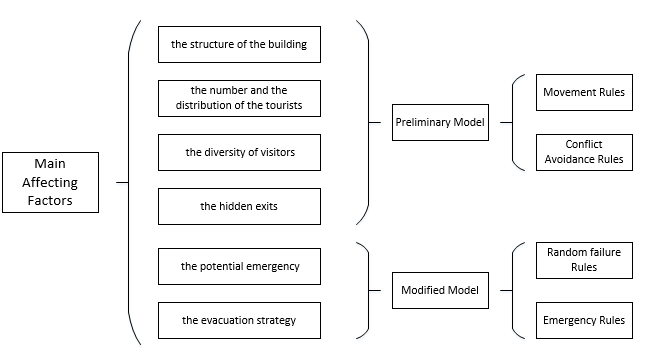
\includegraphics[width=14cm]{1.png}
\end{figure}
\noindent In part I,  we analyse the main factors affecting the evacuation plan, including the structure of the building, the number and the distribution of the tourists, the diversity of visitors, the hidden exits, the potential emergency, as well as the pullout strategy. \\
\indent On the basis of the Cellular Automaton, we set a series of movement rules to imply how these factors  make an impact on the process of leaving  and design the evacuation simulation model.
\subsection{Analysis of Part II}
\begin{figure}[htbp]
%\small
	\centering
	\caption{Recommendations}
	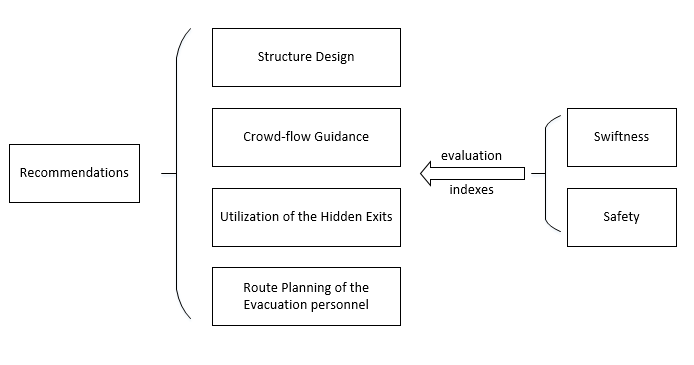
\includegraphics[width=14cm]{2.png}
\end{figure}
\noindent In part II, firstly we define the  evaluation indexes of different evacuation plans, which includes swiftness and safety.\\
\begin{itemize}
	\item Swiftness: All the tourists have to leave the building as quickly as possible.
	\item Safety: The occurrence of emergency should be as less as possible.
\end{itemize}
\quad Assuming that the hazard level is proportional to the degree of crowdedness, the two indexes can be formulated and quantized by the completion time of the plan and the  number of times  that emergency happens respectively. Then we implement the above evacuation simulation model in different situations and compare the results. Based on the comparison, a broad set of options addressing multiple conditions can be made for the design of the pullout plan.
\clearpage
\section{Preliminary Model--Stochastic Cellular Automaton}
\subsection{Basic Theorem of Cellular Automaton}
\begin{figure}[htbp]
%\small
	\centering
	\centering
	\caption{Grid Map}
	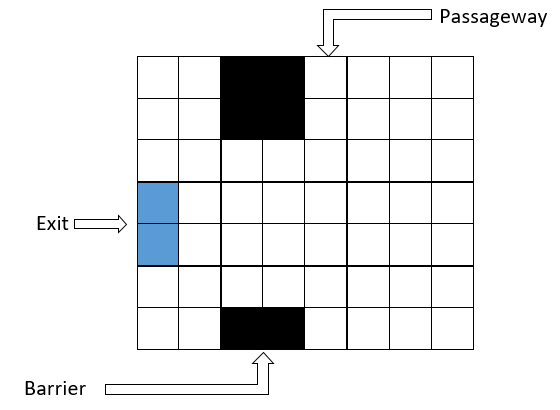
\includegraphics[height=8cm]{4.png}
\end{figure}
\noindent The two-dimmensional Cellular Automaton evenly divides the room into grids, in order to simplify the complex structure into the combination of different grids.[1] The complex structure is classified into three basic grids: exit, barrier and passageway. These basic grids have different degree of position danger as the below formula illustrates and the basic rules is that the cell with higher degree of position danger would move to the cell with lower degree.
\[
	PD(i)=\begin{cases}
		0 & \text{ if } cell_i  is exit  \\
		\infty & \text{ if } cell_i  is barrier  \\
		(x_i-x_0)^2+(y_i-y_0)^2 & \text{ if } cell_i  is passageway
	\end{cases}\eqno (1)
\]
\indent where \(PD(i)\) represents the properties of the grids, \( (x_i,y_i)\) means the current location of the grid while  \( (x_0,y_0)\)  is the location of the exit.\\
\indent When it comes to a signal step, Cellular Automaton utilizes the concept of Moore Neighbourhood, which means each step have nine choices. The probability of choosing one grid is determined by the properties of the grid, as well as the direction.
\begin{figure}[h]
%\small
	\centering
	\caption{Moore Neighbourhood} \label{fig:aa}
	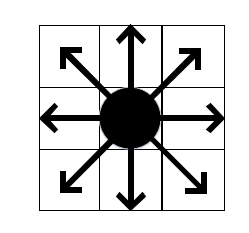
\includegraphics[width=8cm]{5.png}
\end{figure}
\[
	P(i,j)=\begin{cases}
		0 & \text{ if } PD(i,j)=\infty \\
		1 & \text{ if } PD(i,j)=0 \\
		\alpha/9 & \text{ if } 0<PD(i,j)<\infty
	\end{cases}\eqno (2)
\]
\indent where \(P(i,j)\) is the possibility of choosing the grid \(x(i,j)\), \(\alpha\) is related to the direction. \cite{Fu2014}
\subsection{General Assumptions}
\begin{itemize}
	\item For the variety of interests for tourists, the initial distribution of the tourists is in random. Initially, the visitor flow rate of the exhibition hall exceeds that of the normal passageway.
	\item The safety is inversely proportional to the crowdedness of the visitors. The more crowded of the visitors, the more dangerous it would be.
	\item The movement choice of individual tourist is not always optimal. It means, for a signal step, the individual is more possible to choose the optimal route rather than be bounded to choose.
	\item For those who have difficulty in taking care of themselves, like the disabled people, children and the elderly, they have to follow one specified safeguard.
	\item For the tourists in group, they are restricted to keep close to each other and choose the same route.
\end{itemize}
\newpage
\subsection{Notations}
\begin{table}[htbp]
	\begin{tabular}{@{}cl@{}}
		\toprule
		Notations                & Descriptions                                         \\ \midrule
		\((x,y)\)                & Current location                                  \\
		\((i,j)\)                & Possible location of next moment                            \\
		\(P_1(i,j)\)             & Probability of moving to \((i,j)\)                   \\
	\(\lambda_1,\lambda_2)\) & Normalization coefficient                            \\
	\(\mu(i,j)\)             & Status flag of \((i,j)\)                             \\
	\(a(k)\)                 & Psychological endurance of person \(k\)              \\
	\(F_1(i,j)\)             & Location Attraction                                  \\
	\(S(i,j)\)               & Score of \((i,j)\)                                   \\
	\(F_2(i,j)\)             & Conformity tendency                                  \\
	\(P_2(i,j)\)            & Probability of Occupy \((i,j)\)                      \\
	\(b(k)\)                 & Physical strength of person \(k\)                             \\
	\(d(i,j,x,y)\)           & Distance between \((x,y)\) and \((i,j)\)                  \\
	\(\theta\)               & Angle between the last and current movement direction vector\\
	\bottomrule
\end{tabular}
\end{table}
\subsection {Model Design}
\subsubsection{General Framework}
\begin{figure}[htbp]
	\centering
	\caption{General Framework}
	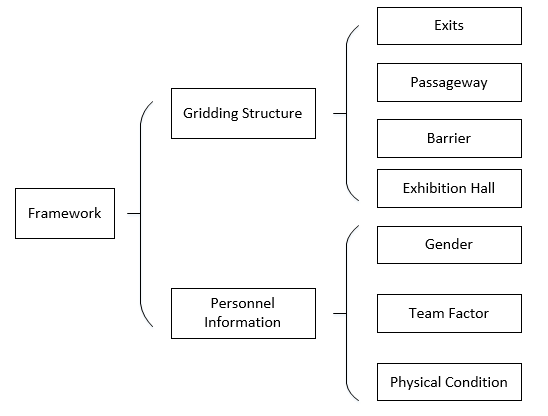
\includegraphics[width=12cm]{3.png}
\end{figure}
\noindent For the preparations of the model, we first model the structure of the building and tourists' information respectively.
\par\indent The structure consists mainly of exhibition hall, passageway and barriers which includes the wall and the fixed roadblock. We intend to utilize the Cellular Automaton, so the floor plan is evenly divided into grids, in size of 0.5m*0.5m. The attributive value of the grid is only determined by whether the grid is occupied by the barrier or the visitor.\\
\indent The information of visitors includes their gender, physical condition and team factor. These information will affect their choice about evacuation route.
\subsubsection{General Movement Rules}
\begin{itemize}
	\item[\textbf {1}] \textbf {Movement Rules}
\end{itemize}
\noindent We classify the tourists into two categories: individual visitors and members of a group. For those who have problem with taking care of themselves or belong to the tourist group, they have to keep a close distance to those belong to the same group and make the uniform choice about escaping route.\\
\indent For one signal cell, the location of next moment is restricted within the adjacent eight cells, which are centered with the current location. We define \((x,y)\)  to represent the current location of cell \(k\), so the moving range for one iteration can be defined as below.
\begin{align}
	i=x-1,x,x+1\\
	j=y-1,y,y+1
\end{align}
\indent The choice is mainly influenced by two factors, the distance and the crowd mentality. The closer the cell \((i,j)\) is to the exit, the more possible that cell would be chosen . We set up variable \(F_1\) to reflect the impacts of the distance, which is called location attraction. Considering that conformity would drive individuals to follow the pace of the surrounding people, we utilize variable \(F_2\) to mirror the potential effects.\\
\indent The combination of group psychology and  psychological endurance codetermine whether one would follow others. Thus, we regard psychological endurance \(\big(a(k),1-a(k)\big)\) as the weight vector of location attraction \(F_1\) and conformity tendency \(F_2\) of cell \(k\) respectively. We set the average level of \(a(k)\) is \( \frac{1}{2} \) and ranges between 0 and 1, obeying normal distribution.
\[
	a(k)\sim\mathrm{N}(\frac{1}{2},\frac{1}{6})
\]
\indent Based on Pauta Creterion, the variance set to \( \frac{1}{6} \) is reasonable because most numerical values of  \(a(k)\) would  meet the requirements of value range.\\
\indent The probability of moving into cell\((i,j)\) from cell\(k\) can be calculated by the following formula.
\[
	P_1(i,j)=\lambda_1\mu(i,j)\Big(a(k)F_1(i,j)+\big(1-a(k)\big)F_2(i,j)\Big)
\]
\indent where \(\mu\) represents the state of the \((i,j)\), whether it is occupied by the barrier or other visitors, \(\lambda\) is the normalization coefficient.
\[
	\mu(i,j)=\left\{\begin{matrix}
			0&\textrm{\quad \; if (i,j) is occupied}\\
			1&\textrm{if (i,j) is blank}
	\end{matrix}\right.
\]
\[
	\sum\limits_{\xi=x-1}^{\xi=x+1}\sum\limits_{\eta=y-1}^{\eta=y+1}P_1(\xi,\eta)=1
\]
\indent Location attraction \(F_1\) can be quantized by the following formula.
\[
	F_1(i,j)=\frac{S_\mathrm{max}-S(i,j)}{S_\mathrm{max}-S_\mathrm{min}}
\]
\indent where \(S(i,j)\) is inversely proportional to the attraction  level of \((i,j)\). Making use of some advanced technology, congestion level of every exit or staircase can be estimated. With longer distance \(d\) or higher congestion level \(\rho\), \(S(i,j)\) would increase rapidly.
\[
	S(i,j)=\rho d
\]
\[
	S_\mathrm{max}=\max\{S(\xi,\eta)|\xi=x-1,x,x+1,\eta=y-1,y,y+1\}
\]
\[
	S_\mathrm{min}=\min\{S(\xi,\eta)|\xi=x-1,x,x+1,\eta=y-1,y,y+1\}
\]
\indent For conformity tendency \(F_2\), the formula can be illustrated as follow.
\[
	F_2(i,j)=\frac{N(i,j)}{\sum\limits_{\xi=x-1}^{x+1}\;\sum\limits_{\eta=y-1}^{y+1}N(\xi,\eta)}
\]
\indent \(N(i,j)\) is the number of people who have passed by \((i,j)\) .
\begin{itemize}
	\item[\textbf {2}] \textbf {Conflict Avoidance Rules}\\
		\noindent If more than one person move to cell \((i,j)\), the conflict will happen. Actually, only one person can enter into the chosen cell while others have to stay at where they were.  Estimation of the probability that person \(k\) successfully occupy the cell \((i,j)\) during confliction can be formulated as below.
\end{itemize}
\[
	P_2(i,j)=\lambda\frac{b(k)}{d(i,j,x,y)}\mathrm{cos}\theta
\]
\[
	b(k)\sim\mathrm{N}(\frac{1}{2},\frac{1}{6})
\]
\begin{figure}[htbp]
	\centering
	\caption{Digraph}
	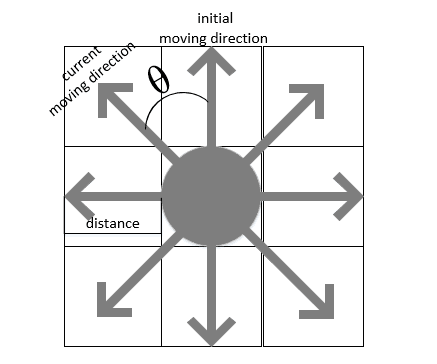
\includegraphics[width=8cm]{digraph.png}
\end{figure}
\par\indent  \quad \( b(k)\): the physical strength factor of person \(k\) and obeys normal distribution.\\
\indent  \quad \(d(i,j,x,y)\): the distance between \((x,y)\) and \((i,j)\).\\
\indent   \quad \(\theta\): the angle between the last movement direction and current movement direction. For the sake of simplification, we use cosine function to indicate the negative relation between the angle and the probability.\\
\section{Modified Model--Emergency Simulation Model}
\subsection{General Assumptions}
\begin{itemize}
	\item The emergency circumstances are classified into two categories: the random confusion and the critical situation.[1]
	\item The occurrence odds of random confusion is negatively correlated to the security level of the site while positively correlated to the crowdedness of the location.
	\item The random confusion will return to normal automatically, which means no need for emergency personnel to enter the site.
	\item The critical situation will occur at any position and the probability is equal.
	\item When the critical situation happens, the emergency personnel have to enter the building to deal with the emergency.
	\item Allowing access for the emergency personnel to enter into the building when the emergency occurs, one tunnel of the exit would be forbidden for the time being and resumes operation after those workers all pass.
\end{itemize}
\newpage
\subsection{Notations}
\begin{table}[htbp]
	\begin{tabular}{@{}cl@{}}
		\toprule
		Notations                & Descriptions                                         \\ \midrule
		\((x,y)\)                & Current location                                \\
		\((i,j)\)                & Possible location of  next moment                        \\
		\(P_3\)                  & Occurrence probability of emergency                 \\
		\(s(i,j)\)               & Danger coefficient of \((i,j)\)                      \\
		\(\rho(i,j)\)            & Population density of \((i,j)\)                      \\
		\(t\) &The increased time when one signal emergency occurs\\
		\(N\)                        & The number of grids which have been occupied by visitors \\
		\(Count\)  &The number of how many times the critical situation occurs\\
		\(T_\textrm{total}\)     & Total lasting time of the evacuation plan                                           \\
		\(T_\textrm{escape}\)    & Lasting time of the evacuation plan                                       \\
		\(T_\textrm{punishment}\)   & Increased time concerning emergency                                 \\ \bottomrule
	\end{tabular}
\end{table}
\subsection{Model Design}
\subsubsection{Random Confusion Model}
\noindent We formulate the possibility of random confusion as below shows.
\[
	P_3(i,j)=s(i,j)\rho(i,j)
\]
\[
	s(i,j)=\left\{\begin{matrix}
			0.001& \textrm{ (i,j) is the main exit}\\
			0.01 \quad& \quad\textrm{(i,j) is the hidden exit}
	\end{matrix}\right.
\]
\[
	\rho(i,j)=\frac{N}{area}  \\
\]
\indent  where area means the acreage surrounding the exit. For simplification, we set the value of area as 25.\\
\indent The impacts of confusion can be defined as below.
\[
	\begin{matrix}
		\mu(i,j,t)=0  \qquad T_{start}\le t \le T_{finish}
	\end{matrix}
\]
\indent where \(T_{start}\) means the moment when the confusion happens while \(T_{finish}\) represents the moment when the confusion terminates.
\subsubsection{Critical Situation Model}
\noindent First we set up the happening probability of critical situations.
\[
	P_3(i,j)=constant
\]
\indent For simplifying, the constant is fixed at 0.001.\\
\indent Then we estimate the potential hazard to the evacuation plan. In order to gain an evaluation criterion  applicable for all the situations, we utilize the punishment time to inflect the effects of safety elements when evaluate the evacuation plan.
\[
	\begin{matrix}
		T_{punishment}=Count \times t   \\
		T_{total}=T_{escape}+T_{punishment}
	\end{matrix}
\]
\indent where \(t_{punishment}\) means the punishment time for one signal time
\section{Evaluation Model}
\noindent Taking the randomness of individual choice and emergency into consideration, it is hardly possible to point out a universal optimal evacuation plan. So we  define two indexes to evaluate different plans: swiftness and safety. They are formulated respectively by the lasting time of the departure process and the occurrence times of emergency. The formula is shown below.
\begin{align}
	&\max\Big(\rho+\frac{1}{t_\textrm{esc}+t_\textrm{res}}+b\Big)\\
	&\textrm{s.t. }
	\left\{
		\begin{aligned}
			&0\leqslant n\leq 4 \\
			&0<\rho < 0.5 \\
			&\rho_{small}\geqslant \rho \\
		\end{aligned}
	\right.
\end{align}
\section{Simplifying and Implementing the Model}
\noindent Intended to apply our model to the Louvre, firstly we have to model the complex structure of the museum. Taken the limitations of calculation ability into consideration, it is hardly possible to simulate the process of numerous tourists evacuating the Louvre, which covers up to 24 hectares. For the evacuation process, the most important factors are the specified structure and the population density. Maintaining the characteristics of structure and the average population density, we simplify the model through decreasing the whole area of the grid structure.\\
\indent The Louvre takes up an area of 480m*172m and receives more than 8 million visitors one year. We simplify the structure into 48 m*17m  and evenly divide the area into grids. Each grid is 0.5m*0.5m, only accommodating one person. The structure model is shown below. The black area represents the barrier, the blue point represents the staircase, the green point means the exit while the purple area is the exhibition hall.
\par\indent The population density is the percentage that the initial number of visitors dividing the maximum number. For the initial population density, we set the value ranges between 0.1 and 0.3, corresponding to the randomness of visitors' number. \\
\indent Then we simulate the process for different conditions and offer a broad set of options in the following section.
\begin{figure}[htbp]
	\centering
	\begin{minipage}[htbp]{10.0cm}
		\centering
		\caption{the ground floor}
		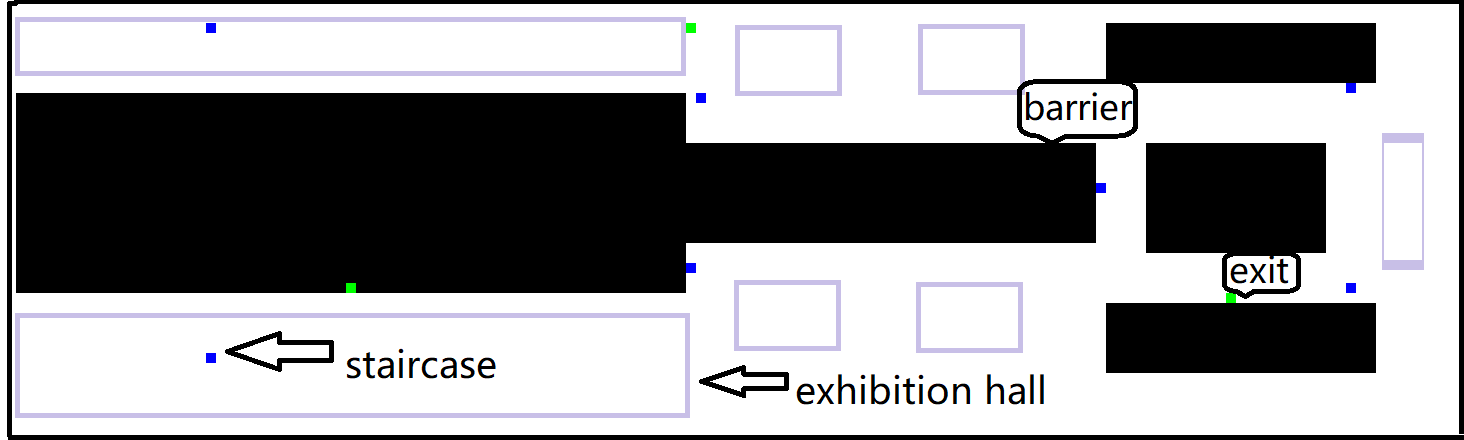
\includegraphics[width=10cm]{0floor.png}
	\end{minipage}
	\begin{minipage}[htbp]{10.0cm}
		\centering
		\caption{the first floor underground}
		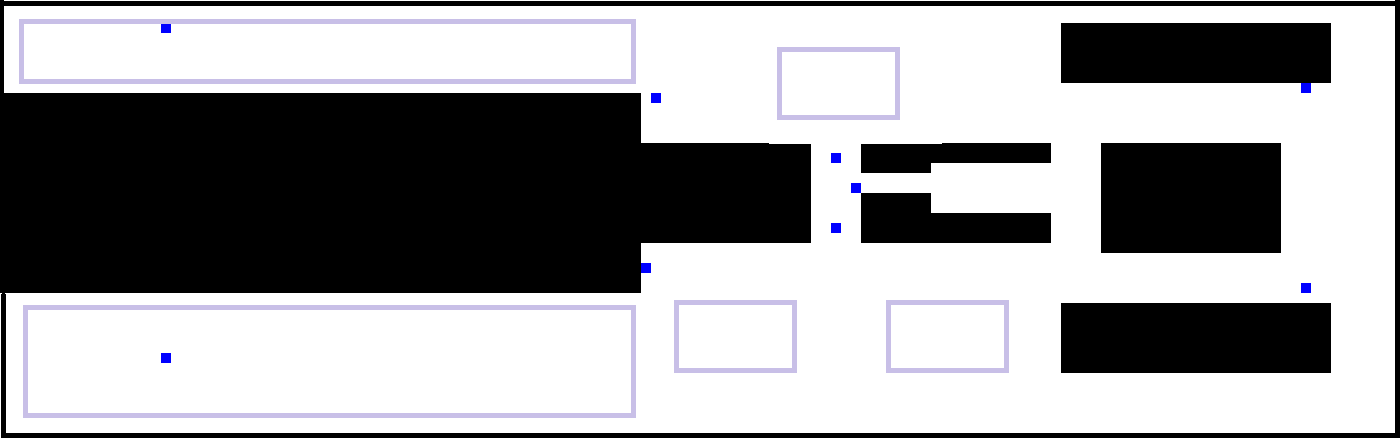
\includegraphics[width=10cm]{-1floor.png}
	\end{minipage}
	\begin{minipage}[htbp]{10.0cm}
		\centering
		\caption{the second floor underground}
		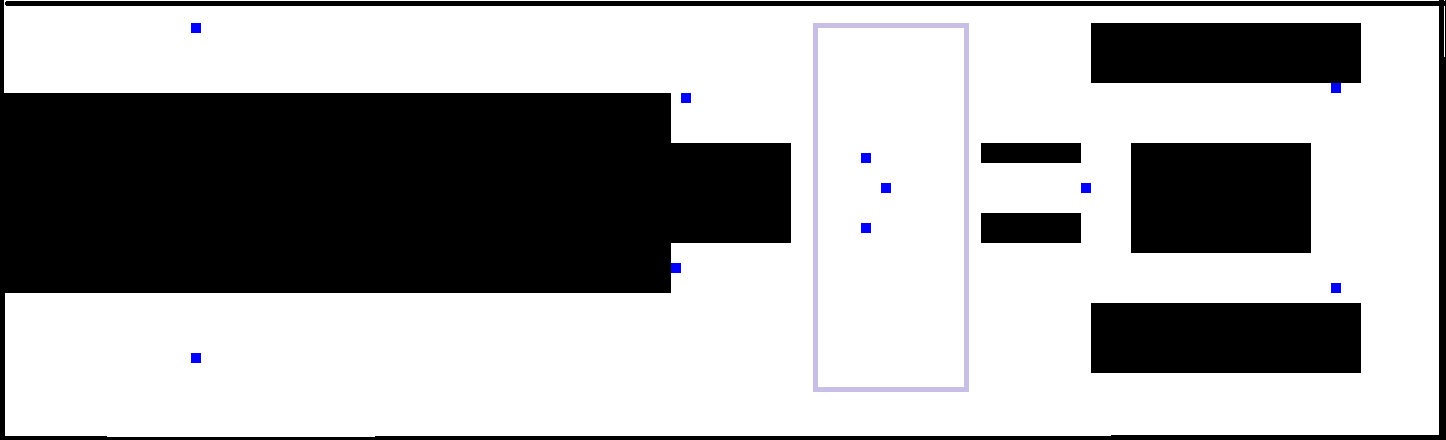
\includegraphics[width=10cm]{-2floor.png}
	\end{minipage}
	\begin{minipage}[htbp]{10.0cm}
		\centering
		\caption{the first floor}
		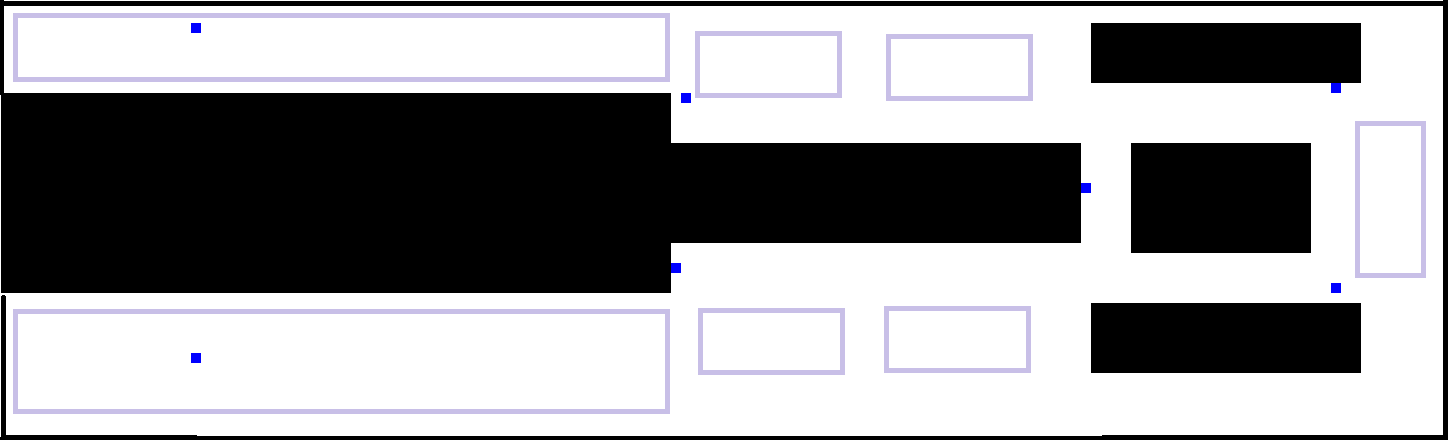
\includegraphics[width=10cm]{1floor.png}
	\end{minipage}
	\begin{minipage}[htbp]{10.0cm}
		\centering
		\caption{the second floor}
		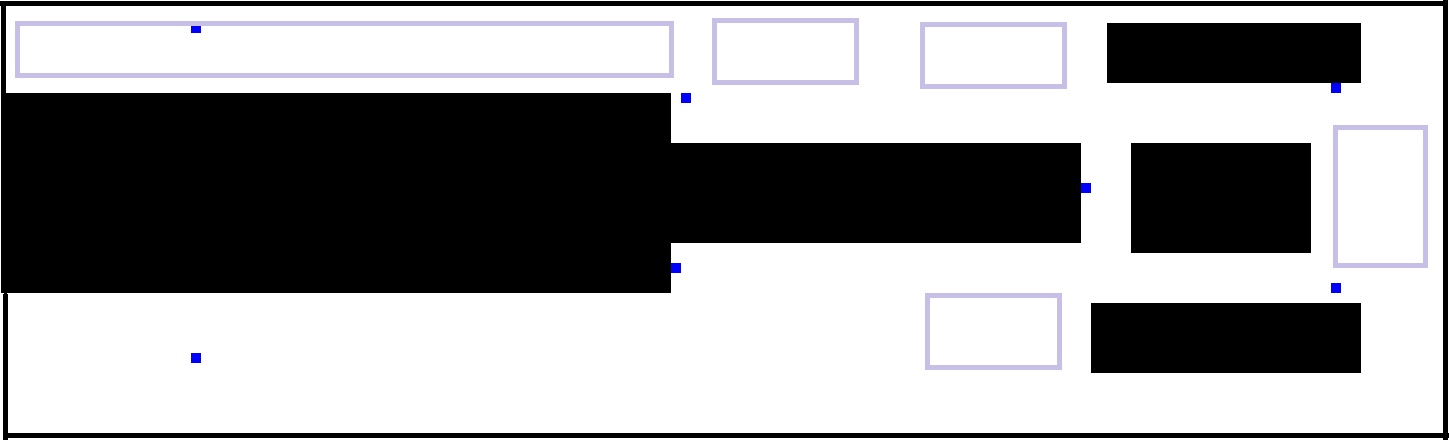
\includegraphics[width=10cm]{2floor.png}
	\end{minipage}
\end{figure}
\clearpage
\section{The Model Results}
\noindent The options mainly consist of four parts: when and how to utilize the hidden exits, the limitations of the maximum tourists' number, smart guidance during evacuation process, the route planning for emergency personnel.
\subsection{Utilizations of the Hidden Exits}
\noindent Assume that some hidden exits [1] distributes in the ground floor, then we determine the optimal site, when to dispark the exit and the reasonable number of open exits.
\subsubsection{Optimal Site}
\noindent The hidden exit may be located near the main exit, the staircase or far away from both the exit and the staircase as the figure x shows. Fix the open strategy and the number of hidden exits, while changing the location. The results is also illustrated below.
\par\indent From the results, the conclusion can be drawn that the optimal site for the hidden exit is away from both the main exit and the staircase. In this situation, the crowdedness of visitors is significantly decreased, resulting in lower occurrence possibility of confusion and speeding up the process.
\begin{figure}[htbp]
%\small
	\centering
	\begin{minipage}[htbp]{10.0cm}
		\centering
		\caption{additional exit nearby the exit}
		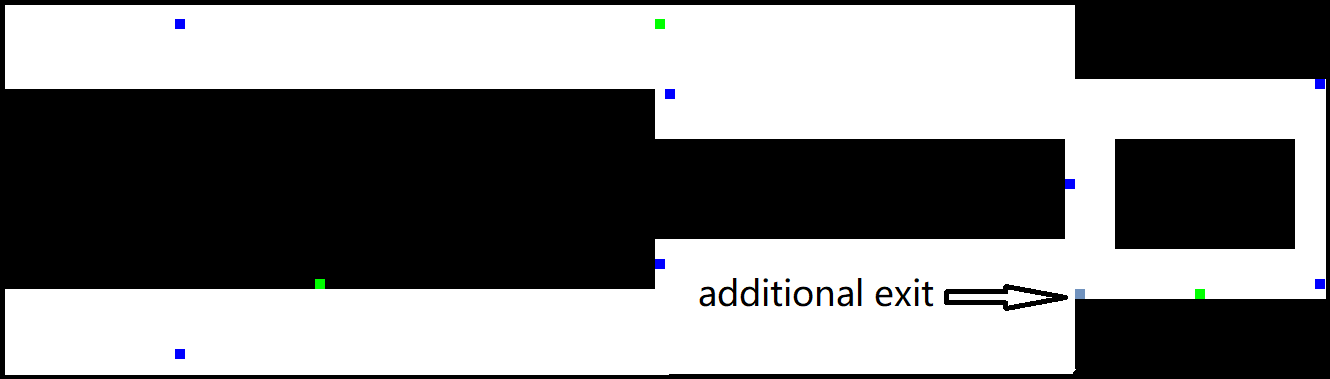
\includegraphics[width=10cm]{smalldoor1.png}
	\end{minipage}
	\begin{minipage}[htbp]{10.0cm}
		\centering
		\caption{process}
		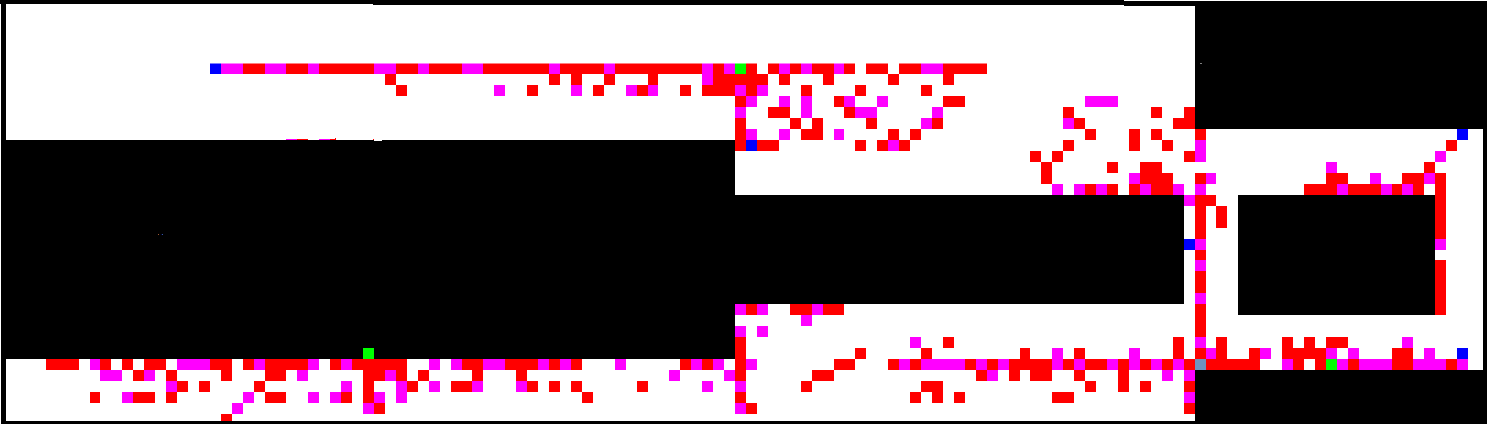
\includegraphics[width=10cm]{smalldoor1_run.png}
	\end{minipage}
\end{figure}
\begin{figure}[htbp]
%\small
	\begin{minipage}[htbp]{10.0cm}
		\centering
		\caption{additional exit nearby the staircase}
		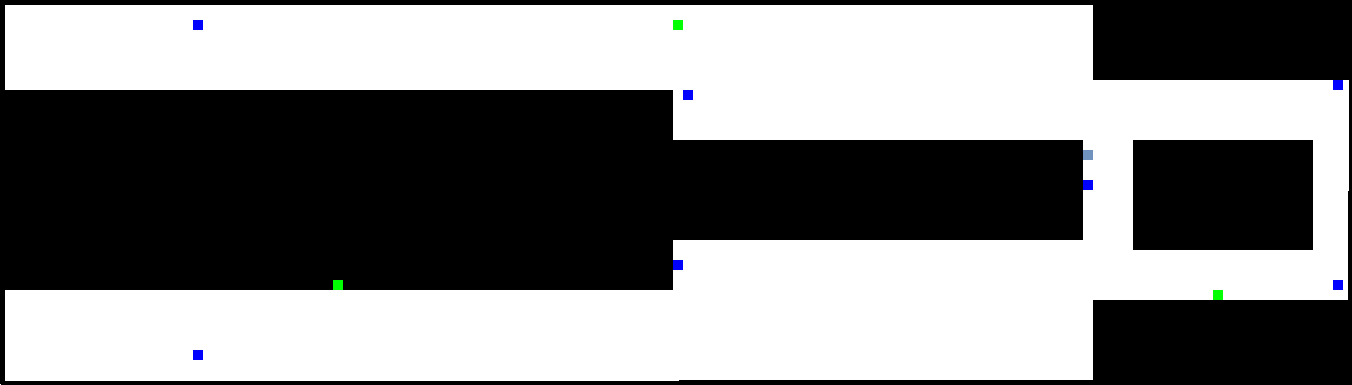
\includegraphics[width=10cm]{smalldoor2.png}
	\end{minipage}
%\small
	\centering
	\begin{minipage}[htbp]{10.0cm}
		\centering
		\caption{process}
		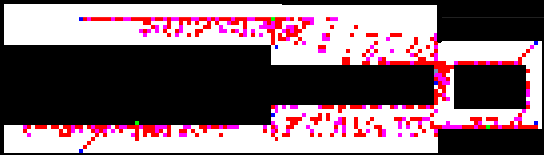
\includegraphics[width=10cm]{smalldoor2_run.png}
	\end{minipage}
	\begin{minipage}[htbp]{10.0cm}
		\centering
		\caption{additional exit away from the exit and the staircase}
		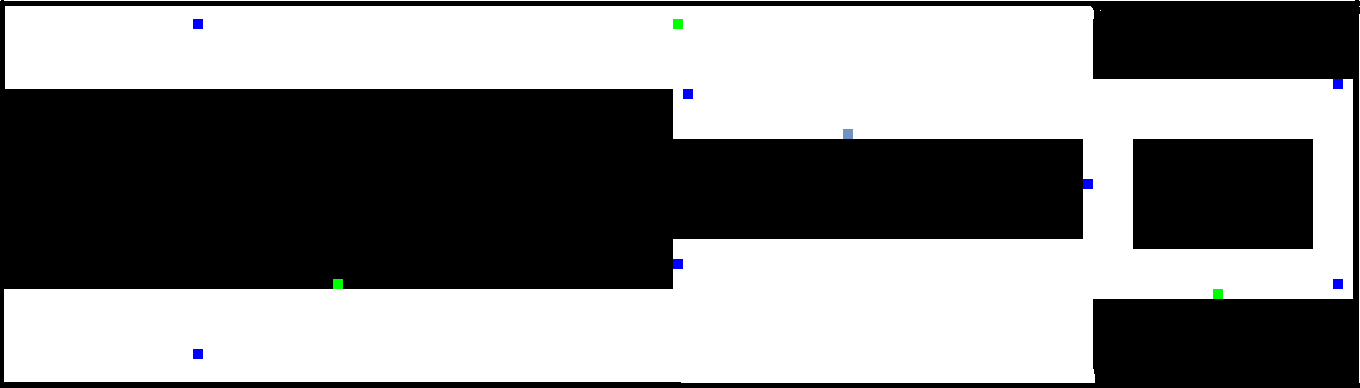
\includegraphics[width=10cm]{smalldoor3.png}
	\end{minipage}
	\begin{minipage}[htbp]{10.0cm}
		\centering
		\caption{process}
		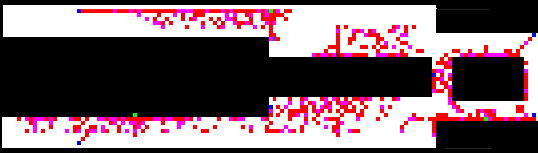
\includegraphics[width=10cm]{smalldoor3_run.png}
	\end{minipage}
\end{figure}
\newpage
\subsubsection{When to Dispark the Exit}
\noindent When it comes to when to open the hidden exit, there are two basic methods: no restrictions and only dispark it.
\begin{table}[htbp]
	\caption{no restrictions}
	\begin{tabular}{@{}ccccc@{}}
		\toprule
		\begin{tabular}[c]{@{}c@{}}Population\\   density\end{tabular}                          & \begin{tabular}[c]{@{}c@{}}Percentage of building capacity\\   to accommodate the largest number of people\end{tabular} & 0.1 & 0.2 & 0.3 \\ \midrule
		\multirow{6}{*}{\begin{tabular}[c]{@{}c@{}}Time(s)(No Rescue\\   Channel)\end{tabular}} & Three exits                                                                                                             & 293 & 312 & 354 \\
		&One additional door (nearby stairs)                                                                                             & 261 & 292 & 332 \\
		&One additional door (nearby exit)                                                                                               & 272 & 273 & 322 \\
		& \begin{tabular}[c]{@{}c@{}}One additional doors (away from stairs and\\   exits)\end{tabular}                               & 230 & 271 & 318 \\\bottomrule
	\end{tabular}
\end{table}
\begin{table}[htbp]
	\caption{with restrictions}
	\begin{tabular}{@{}ccccc@{}}
		\toprule
		\begin{tabular}[c]{@{}c@{}}Population\\   density\end{tabular}                          & \begin{tabular}[c]{@{}c@{}}Percentage of building capacity\\   to accommodate the largest number of people\end{tabular} & 0.1 & 0.2 & 0.3 \\ \midrule
		\multirow{7}{*}{\begin{tabular}[c]{@{}c@{}}Time(s)(No Rescue\\   Channel)\end{tabular}} & Three exits                                                                                                             & 293 & 312 & 354 \\
		&One additional door (nearby stairs)                                                                                             & 270 & 289 & 338 \\
		&One additional door (nearby exit)                                                                                               & 261 & 279 & 317 \\
		& \begin{tabular}[c]{@{}c@{}}One additional doors (away from stairs and\\   exits)\end{tabular}                               & 245 & 262 & 309 \\\bottomrule
	\end{tabular}
\end{table}
\subsection{Limitations of the Maximum Visitors}
\noindent The number of the visitors should be limited at at reasonable level. Considering that the earnings is in positive relation to the number of visitors while the evacuation efficiency is in negative relation to that. To trade off the two factors, we introduce the maximum area theorem: plot the two variable in one picture, the optimal solution corresponds to the maximum section area.  \\
\indent As the figure below illustrates, the optimal population density is 0.36.
\begin{figure}[htbp]
	%\small
	\centering
	\caption{Maximum Visitors}
	\includegraphics[width=9cm]{result.eps}
\end{figure}
\subsection{Reasonable Distribution of Exhibition Hall}
\noindent As the below figures shown, the initial distribution of the visitors is related to that of the exhibition halls. For some floors, the uneven distribution of exhibition halls leads to overcrowding and does harm to the evacuation process.
\indent Compare the results of even distribution and the uneven distribution, the conclusion can be drawn that the exhibition halls are supposed to evenly distribute during the floor plane.
\begin{table}[htbp]
	\centering
	\begin{tabular}{@{}ccc@{}}
		\toprule
		population density & Actual distribution & uniform distribution \\\midrule
		0.2                & 312                 & 276                 \\\bottomrule
	\end{tabular}
\end{table}
\subsection{Route Planning for the Emergency Personnel}
\noindent The route plans of emergency personnel are divided into two categories: the path in the shortest distance and the least crowded route. Comparing the results shown below, we conclude that when the population density is less than 0.48, the route in the shortest distance may speed up the process. Inversely, the route of least crowdedness may be better.
\begin{figure}[htbp]
	%\small
	\centering
	\begin{minipage}[htbp]{10.0cm}
		\centering
		\caption{even distribution figure}
		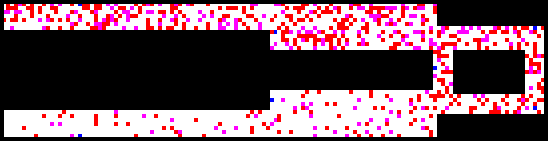
\includegraphics[width=10cm]{result3.png}
	\end{minipage}
	\begin{minipage}[htbp]{10.0cm}
		\centering
		\caption{uneven distribution}
		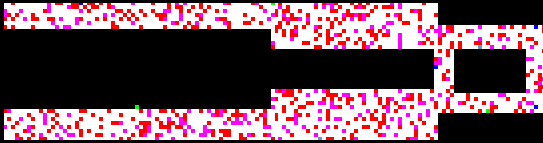
\includegraphics[width=10cm]{result4.png}
	\end{minipage}
\end{figure}
\begin{figure}[htbp]
%\small
	\caption{Route Planning}
	\centering
	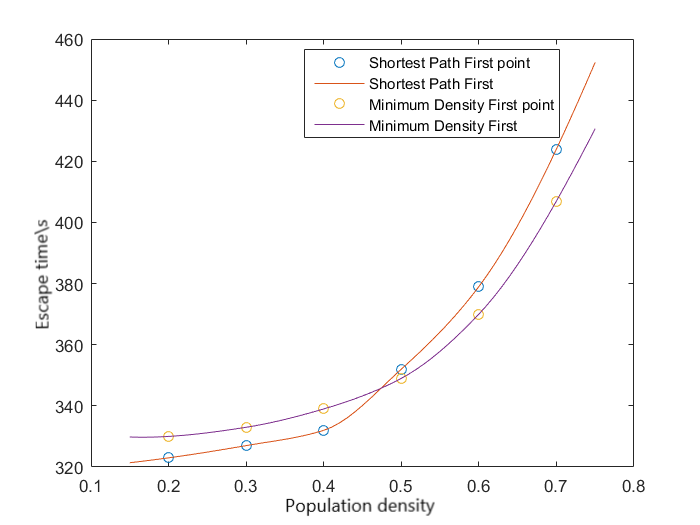
\includegraphics[width=10cm]{result2.png}
\end{figure}
\section{Validation and Prospect of the Model}
\noindent To validate the practicability of our model, we compare our results with the actual experiments.\\
\indent Shanshan Mao (2018)[2] conducted experiments on a  primary school and timed the evacuation process.The following is her experimental results.\\
\begin{table}[htbp]
	\centering
	\caption{Experiment Results}
	\begin{tabular}{@{}ccc@{}}
		\toprule
		Time   & No guidance & With guidance     \\ \midrule
		first  & 110 s  & 92 s        \\
		second & 106 s  & 89 s        \\
		third  & 113 s  & 90 s        \\ \bottomrule
	\end{tabular}
\end{table}
\par\indent Utilizing our system, we first model the structure of the primary school, with two floors. Then we estimate the leaving process based on the structure model and achieve the final results. The only difference of the conditions is whether adopt the suggestions we suggest above. The model and results are shown below. To simplify the calculation, we assume the structure for three floors is the same. As the figure 6 shows, the blue area is the door or staircase while the pink area is the classroom.\\
\begin{figure}[htbp]
%\small
	\centering
	\begin{minipage}[htbp]{10.0cm}
		\centering
		\caption{Structure Model}
		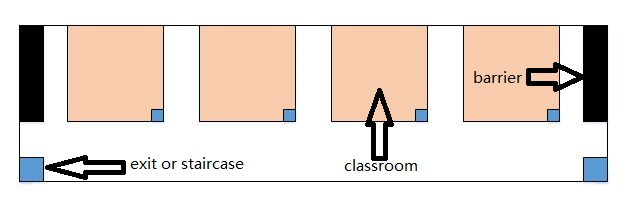
\includegraphics[width=10cm]{6.jpg}
%\begin{table}
	\end{minipage}
	\begin{minipage}[htbp]{8.0cm}
		\centering
		\caption{Simulation Results}
		\begin{tabular}{@{}cccll@{}}
			\toprule
			Time   & No guidance & With guidance &  &  \\ \midrule
			first  & 150 s  & 132 s    &  &  \\ \bottomrule
		\end{tabular}
	\end{minipage}
%\end{table}
\end{figure}
\par\indent From the comparison of the results, we could come to the conclusion that the results is close to the actual situation for we considering comprehensively. \\
\indent The example implementation of our model validates that the system is applicable and is convenient to apply to other structures.
\section{Evaluation of the Model}
\subsection{Sensitivity Analysis}
The figure illustrates the relation between the population density and the total lasting time of the leaving process. The conclusion can be drawn that the results is sensitive to the change of the population density, corresponding to the reality.
\begin{figure}[htbp]
		\centering
		\caption{Sensitivity}
		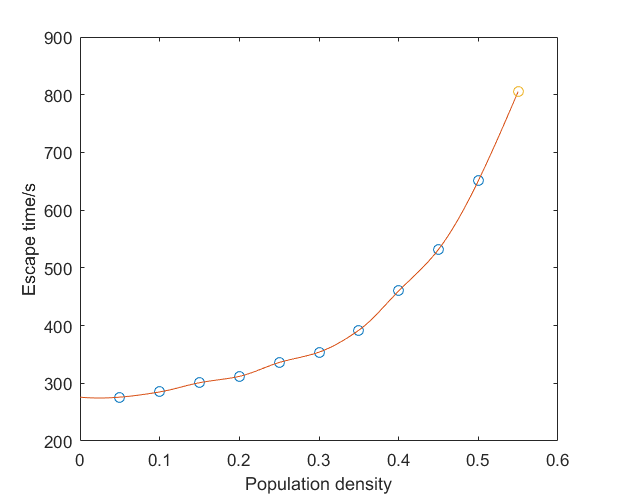
\includegraphics[width=10cm]{sensitivity.png}
\end{figure}
\subsection{Strengths}
\begin{itemize}
	\item \textbf{Applicable}\\
		Taking a broad set of affecting factors into consideration, this system can apply to various types of public structures, and the information of visitors is approximately the same. The only operation is to model the structure for the specific structure, making it convenient to implement the model.
	\item \textbf{Reasonable Simplification}\\
		With reasonable simplification, we focus on the specific structure of the building rather than be confined to the huge area and masses of
		individuals. Introduce the concept of population density, we achieve the goal of reducing area of the building and the number of visitors while maintain the population density.
	\item \textbf{Multiple Solutions}\\
		Taking account of the randomness of the initial distribution of visitors and the occurrence of emergency, it is nearly impossible to offer an optimal solution which is applicable to different situations. So we explore multiple options to address various conditions.
\end{itemize}
\subsection{Weakness}
\begin{itemize}
	\item \textbf{Randomness}\\
		The process of cellular automaton is in random, so the estimation is lack of accuracy. Optimizing the parameters, like the diversity of visitors, through the statistical data, the  estimation can be close to the actual conditions.
	\item \textbf{Limitations}\\
		The iteration of our system is limited to the local optimum, thus may leads to inaccuracy. Given the possible existence of command system, apart from the blindness of visitors, the effects of guidance should be taken into consideration.
\end{itemize}
\section{A Memo to the Louvre Museum Leaders}
To: The Museum Leaders\\
From: ICM team \\
Re: Emergency Evacuation Simulation Model Based on Cellular Automata \\\\
Dear Sir/Madam:\\\\
\indent We have heard of your organization's worries about the evacuation plan to address the emergency, so we set up a evacuation simulation model to offer you our assistance. We are a team of students who have dedicated four intense days to explore a broad set options dealing with various conditions for you to select. While many have been working on this field for years, we still believe that our approach will give you extra help you are seeking.\\
\indent In order to explore the preferable solutions, we first build the evacuation simulation model based on the two-dimensional cellular automaton. The main affecting factors of the leaving process are the structure of building and the detailed information of visitors. For the architecture, we regard the building as the combination of exits, barriers and staircases. Evenly divide the building plane into grids and endow them with different numerical values according to the location. With regard to the information of tourists, we select three main factors: physical conditions, age and gender, as well as whether a member of one group. The simulation is completed by the continual iterations of the grids' properties. For the iteration, we set several rules to emulate the actual movement of people, including movement rules, conflict avoidance rules and the emergency rules. \\
\indent Taking the randomness of individual choice and emergency into consideration, it is hardly possible to point out a universal optimal evacuation plan. So we define two indexes to evaluate different plans: swiftness and safety. They are formulated respectively by the lasting time of the departure process and the occurrence times of emergency. The evaluation model is the combination of the two indexes. \\
\indent Utilizing the simulation model and the evaluation criteria set up above, we explore a broad set of options for various conditions. For the implementation of the Louvre, we offer four specific suggestions, consisting of the maximum number of visitors, the reasonable distribution of exhibition halls, the strategy to utilize the hidden exits as well as the route planning of the emergency personnel. \\
\indent Specifically, first is the utilization of the additional hidden exits. From comparison, the optimal location is away from the main exit or staircase. The reasonable moment to open up that is determined by the population density: only dispark the hidden exit when the density is less than 0.5. What's more, when the number of exits reaches up to two, the lasting time of escaping process is the least wile maintain low possibly of emergency. \\
\indent Secondly, when it comes to the limitations of the maximum visitors, we consider two factors: the earnings and the effects of the evacuation plan. Trading off the two factors, we suggest that it is reasonable to set the maximum population density at 0.39. \\
\indent Thirdly, with regard to the distribution of exhibition halls, we propose that evenly distribute the exhibition halls to avoid overcrowding in some sites. \\
\indent Fourthly, the route for emergency personnel entering the site where the emergency occurs is determined by the population density. If the density less than 0.19, the optimal route is the shortest distance between the emergency personnel and the location where emergency happens, while the optimal route is the least crowdedness if the density exceeds 0.19.\\\\

Sincerely\\
\quad ICM Team\\
\clearpage
\bibliographystyle{ieeetr}
\begin{thebibliography}{99}
\bibitem{1}.S. Zhou and J. Meng An Improved Algorithm of the Cellular Automata on the Evacuation Simulation[J]. Physica A:  Statistical Mechanics and its Applications, 2001, 295(1). Publishing Company, 1984-1986.
\bibitem{2}Shanshan Mao. Research on evacuation model in elementary and middle school based on Cellular Automata[D]. Nankai University, 2010.
\end{thebibliography}
\bibliography{main}
\begin{appendices}
	\section{Code}
	\lstinputlisting[language=Matlab]{code/test.m}
	\lstinputlisting[language=Matlab]{code/same.m}
	\lstinputlisting[language=Matlab]{code/find_chukou.m}
	\lstinputlisting[language=Matlab]{code/ditu.m}
	\lstinputlisting[language=Matlab]{code/ditu1.m}
	\lstinputlisting[language=Matlab]{code/ditu2.m}
	\lstinputlisting[language=Matlab]{code/cal_den.m}
	\lstinputlisting[language=Matlab]{code/cal_distance.m}
\end{appendices}
\end{document}
